\documentclass[12pt,a4paper]{article}
\usepackage{amsmath,amscd,amsbsy,amssymb,latexsym,url,bm,amsthm}
\usepackage{epsfig,graphicx,subfigure}
\usepackage{enumitem,balance}
\usepackage{wrapfig}
\usepackage{mathrsfs,euscript}
\usepackage[usenames]{xcolor}
\usepackage{hyperref}
\usepackage[vlined,ruled,linesnumbered]{algorithm2e}
\usepackage{float}
\hypersetup{colorlinks=true,linkcolor=black}

\newtheorem{theorem}{Theorem}
\newtheorem{lemma}[theorem]{Lemma}
\newtheorem{proposition}[theorem]{Proposition}
\newtheorem{corollary}[theorem]{Corollary}
\newtheorem{exercise}{Exercise}
\newtheorem*{solution}{Solution}
\newtheorem{definition}{Definition}
\theoremstyle{definition}

\renewcommand{\thefootnote}{\fnsymbol{footnote}}

\newcommand{\postscript}[2]
{\setlength{\epsfxsize}{#2\hsize}
	\centerline{\epsfbox{#1}}}

\renewcommand{\baselinestretch}{1.0}

\setlength{\oddsidemargin}{-0.365in}
\setlength{\evensidemargin}{-0.365in}
\setlength{\topmargin}{-0.3in}
\setlength{\headheight}{0in}
\setlength{\headsep}{0in}
\setlength{\textheight}{10.1in}
\setlength{\textwidth}{7in}
\makeatletter \renewenvironment{proof}[1][Proof] {\par\pushQED{\qed}\normalfont\topsep6\p@\@plus6\p@\relax\trivlist\item[\hskip\labelsep\bfseries#1\@addpunct{.}]\ignorespaces}{\popQED\endtrivlist\@endpefalse} \makeatother
\makeatletter
\renewenvironment{solution}[1][Solution] {\par\pushQED{\qed}\normalfont\topsep6\p@\@plus6\p@\relax\trivlist\item[\hskip\labelsep\bfseries#1\@addpunct{.}]\ignorespaces}{\popQED\endtrivlist\@endpefalse} \makeatother

\begin{document}
	\noindent
	
	%========================================================================
	\noindent\framebox[\linewidth]{\shortstack[c]{
			\Large{\textbf{Lab05-DynamicProgramming}}\vspace{1mm}\\
			CS214-Algorithm and Complexity, Xiaofeng Gao, Spring 2021.}}
	\begin{center}
		\footnotesize{\color{red}$*$ If there is any problem, please contact TA Haolin Zhou.}
		
		% Please write down your name, student id and email.
		\footnotesize{\color{blue}$*$ Name:Yanjie Ze  \quad Student ID:519021910706 \quad Email: zeyanjie@sjtu.edu.cn}
		
	\end{center}
	
	\begin{enumerate}
		\item \textit{Optimal Binary Search Tree.} Given a sorted sequence $K=\left \langle k_{1}, k_{2}, \ldots, k_{n} \right \rangle$ of $n$ distinct keys, and we wish to build a binary search tree from these keys. For each key $k_{i}$, we have a probability $p_{i}$ that a search will be for $k_{i}$. Some searches may be for values not in $K,$ and so we also have $n+1$ \emph{dummy keys} $d_{0}, d_{1}, d_{2}, \ldots, d_{n}$ representing values not in $K$. In particular, $d_{0}$ represents all values less than $k_{1}$, and $d_{n}$ represents all values greater than $k_{n}$. For $i=1,2, \ldots, n-1,$ the dummy key $d_{i}$ represents all values between $k_{i}$ and $k_{i+1}$. For each dummy key $d_{i}$, we have a probability $q_{i}$ that a search will correspond to $d_{i}$. Each key $k_{i}$ is an internal node, and each dummy key $d_{i}$ is a leaf. Every search is either successful (finding some key $k_{i}$ ) or unsuccessful (finding some dummy key $d_{i}$ ), and so we have $ \sum_{i=1}^{n} p_{i}+\sum_{i=0}^{n} q_{i}=1 $. 
		\begin{enumerate}
			\item Prove that if an optimal binary search tree $T$ ($ T $ has the smallest expected search cost) has a subtree $T^{\prime}$ containing keys $k_{i}, \ldots, k_{j},$ then this subtree $T^{\prime}$ must be optimal as well for the subproblem with keys $k_{i}, \ldots, k_{j}$ and dummy keys $d_{i-1}, \ldots, d_{j}$. 
			
			\begin{solution}
			~\\
			Denote $E(cost^*)$ as the smallest expected search cost of an optimal binary search tree $T$ containing keys $k_1,k_2,...,k_n$ and dummy keys $d_0, d_1, ..., d_n$.
			
			Denote $E(subcost^*)$ as the smallest expected search cost of an optimal binary search tree $T'_{opt}$ containing keys $k_i,...,k_j$ and dummy keys $d_{i-1},...,d_j$ and denote $E(subcost)$ as the expected search cost of a binary search tree $T'_{norm}$ covering the same keys as $T$, but $T'_{norm}$ is not optimal though. 
			
			By definition, $E(subcost^*)<E(subcost)$.
			
			~\\
			To search an element ranging from $d_{i-1}$ to $d_j$, we can divide this into 2 subproblems:
			
			\begin{itemize}
			    \item Reach the subtree. Assume the cost of reaching the subtree from the root is $C$.
			    
			    \item Search in the subtree. The cost depends on the subtree.
			\end{itemize}
			
			~\\
			\textbf{One key problem here is: Whether $C$ is the same for both subtrees?} 
			
			The answer is YES.
			
			Let's assume the cost $C$ is not the same, which means:
			although the normal subtree's expected cost is more than the optimal, its $C$ is less than $C$ of the optimal subtree. As shown in Fig.~\ref{tree1} and Fig.~\ref{tree3}, although the optimal subtree costs less in itself, there needs larger cost $C$ to reach the optimal subtree, while in Fig.~\ref{tree3}, the subtree is not optimal but it has smaller cost $C$. The situation seems to be hard to judge.
			
			\textbf{However}, this is not possible. Because if the normal subtree in Fig.~\ref{tree3} exists, this subtree will certainly be improved to an optimal one, as shown in Fig.~\ref{tree4}.
			
			\textbf{Therefore, the cost of reaching the subtree for a normal subtree $T'_{norm}$ and its corresponding optimal subtree $T'_{opt}$, $C$, should be the same.}
			
			
			
           \begin{figure}[htbp]
            \centering
            \begin{minipage}[t]{0.48\textwidth}
            \centering
            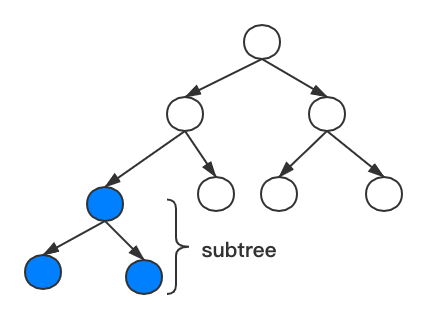
\includegraphics[width=6cm]{Lab05-YanjieZe/tree1.png}
            \caption{Optimal Subtree}\label{tree1}
            \end{minipage}
            \begin{minipage}[t]{0.48\textwidth}
            \centering
            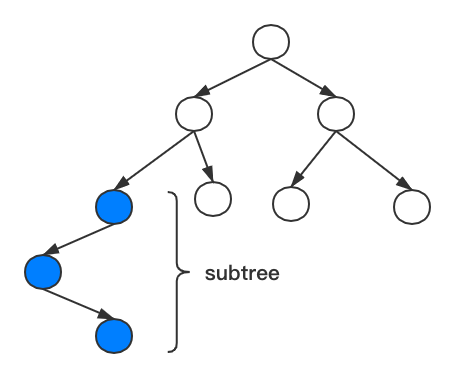
\includegraphics[width=6cm]{Lab05-YanjieZe/tree2.png}
            \caption{Normal Subtree}\label{tree2}
            \end{minipage}
            \end{figure}

			~\\
			Then we prove the subtree should be optimal.
			
			If $T$'s subtree is not optimal, assume it is $T'_{norm}$, as shown in Fig.~\ref{tree2}, then:
			$$
			E(cost^*) = E(subcost) + C > E(subcost^*) + C
			$$
			Which means $T$ is not optimal, leading to a contradiction.
			
			Therefore, the subtree of $T$ should be optimal, and  naturally the subtree is optimal for the subproblems with keys $k_i,...,k_j$ and dummy keys $d_{i-1},...,d_j$.
			
	
                \begin{figure}[htbp]
            \centering
            \begin{minipage}[t]{0.48\textwidth}
            \centering
            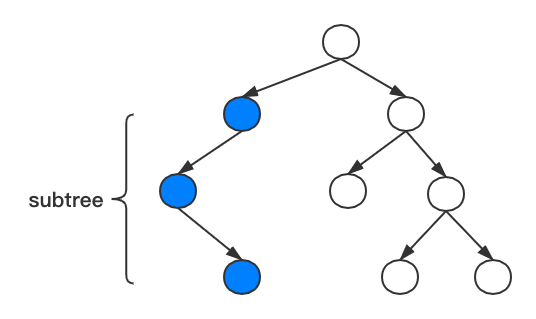
\includegraphics[width=6cm]{Lab05-YanjieZe/tree3.png}
            \caption{Is $C$ the same?(1)}\label{tree3}
            \end{minipage}
            \begin{minipage}[t]{0.48\textwidth}
            \centering
            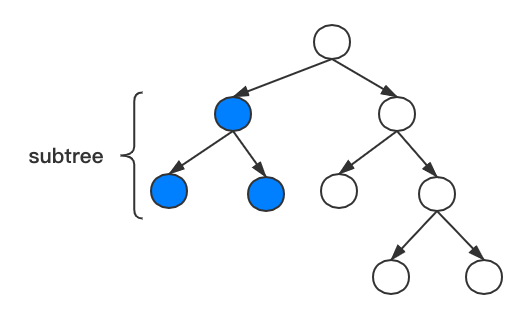
\includegraphics[width=6cm]{Lab05-YanjieZe/tree4.png}
           \caption{Is $C$ the same?(2)}\label{tree4}
            \end{minipage}
            \end{figure}
            
			\end{solution}
			
			\item We define $e[i, j]$ as the expected cost of searching an optimal binary search tree containing the keys $k_{i}, \ldots, k_{j} .$ Our goal is to compute $e[1, n]$. Write the state transition equation and pseudocode using \textbf{dynamic programming} to find
			the minimum expected cost of a search in a given binary tree. (\textbf{Remark}: You may use $ w(i, j)=\sum_{l=i}^{j} p_{l}+\sum_{l=i-1}^{j} q_{l} $).
			
			\begin{solution}
			~\\
			Denote $r$ as the root of the subtree.
			
			Denote $w(i, j)=\sum_{l=i}^{j} p_{l}+\sum_{l=i-1}^{j} q_{l}$, as the probability of reaching root $r$ from last node. 
			
			Then we can divide the calculation of $e[i,j]$ into subproblems: \begin{itemize}
			    \item Figure out every $e[i,r-1]$ and $e[r+1, j]$, for $i\leq r \leq j$.
			    \item Find $r$ that can minimize $e[i,r-1] + e[r+1,j] + w[i,j]$.
			\end{itemize}
			
			Therefore, we have such state transition equation:
			
			$$ 
			e[i,j]=\left\{
            \begin{aligned}
            &0,\quad &when\quad i-j>1\\
            &q_j,\quad &when\quad i-j=1\\
            &\min_{i\leq r\leq j}\{ e[i,r-1] + e[r+1, j] + w[i,j]\},\quad &when\quad i\leq j
            \end{aligned}
            \right.
            $$
            
            ~\\
            
            
            \textbf{Another essential problem is how we calculate $e[i,j]$ in a bottom-up manner.} 
            
            It's acknowledged that the brute force algorithm is much time-consuming, thus we need to figure out a tabular method.
            
            Obviously:
                \begin{equation}
                \begin{split}
                \label{eq1}
                e[i,i] &= e[i,i-1] + e[i+1, i] + w[i,i]\\
                    &= q[i-1] + q[i] + w[i,i]
                 \end{split}       
                \end{equation}
                
            So we first compute these $e[i,i]$ using the formula~\ref{eq1}, as shown in Fig.~\ref{axis1}. In Fig.~\ref{axis1}, {\color{red} the red dots} represent these computed $e[i,j]$.
            ~\\
            
  
            Then taking $e[1,2]$ as the example, we show what can be computed next step.
            
            \begin{equation}
                \begin{split}
                    \label{eq2}
                    e[1,2]&=min\{e[1,0]+e[2,2]+w[1,2], e[1,1]+e[3,2]+w[1,2]\}\\
                    &=min\{ q_0+e[2,2]+w[1,2], q_2+e[1,1]+w[1,2]\}
                \end{split}
            \end{equation}
            
            Similarly, we can compute $e[i,i+1]$ next step, based on $e[i,i]$ and $e[i+1,i+1]$, so we have Fig.~\ref{axis2}.{\color{blue}The blue dots} represent these computed $e[i,i+1]$ and the dotted lines between them represent the connection of computation.
            
              \begin{figure}[htbp]
            \centering
            \begin{minipage}[t]{0.48\textwidth}
            \centering
            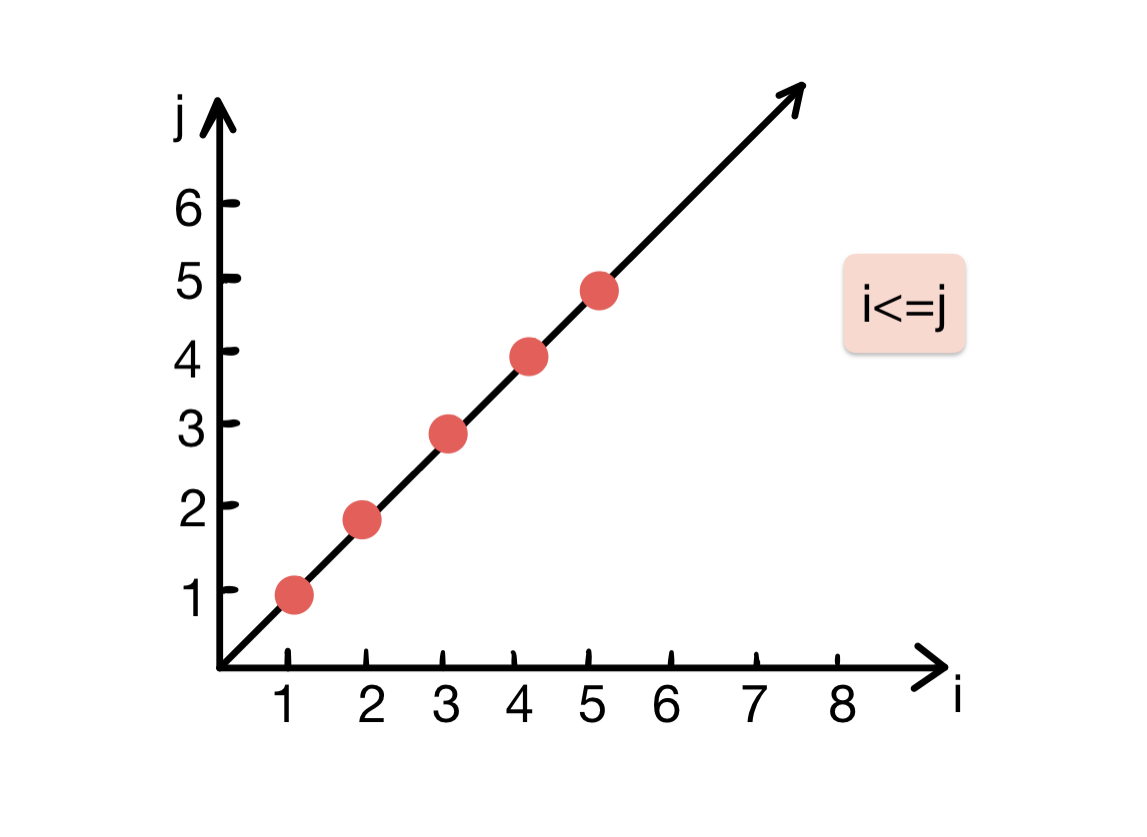
\includegraphics[width=6cm]{Lab05-YanjieZe/axis1.jpg}
           \caption{Compute $e[i,i]$}\label{axis1}
            \end{minipage}
            \begin{minipage}[t]{0.48\textwidth}
            \centering
            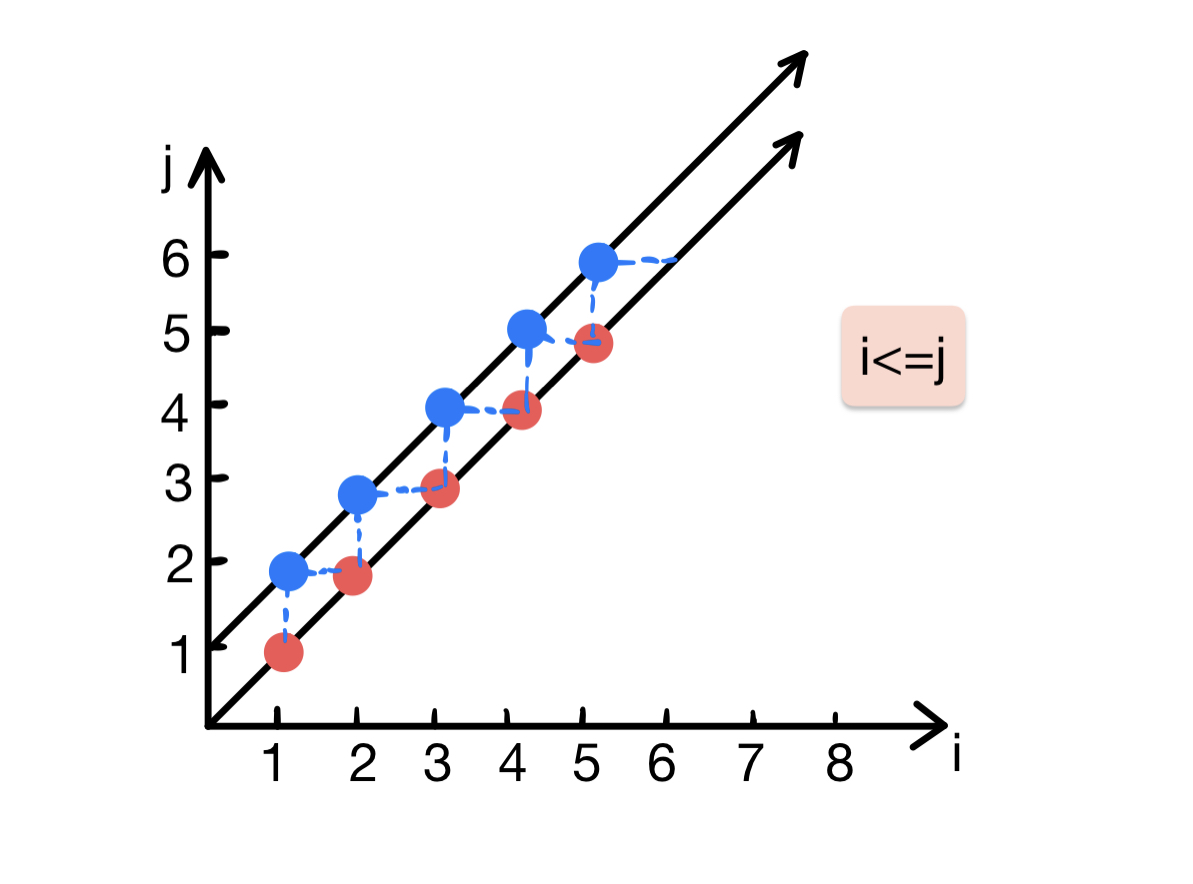
\includegraphics[width=6cm]{Lab05-YanjieZe/axis2.jpg}
            \caption{Compute $e[i,i+1]$}\label{axis2}
            \end{minipage}
            \end{figure}
            
            Finally, we are able to conclude the correct computation path of $e[i,j]$, shown in Fig.~\ref{axis3}. We start from calculating each $e[i,i]$, then each $e[i,i+1]$, each $e[i,i+2]$, ... Intuitively, this computation path is the same as {\color{orange}the colorful line}.
            
            
            \begin{figure}[htbp]
                \centering
                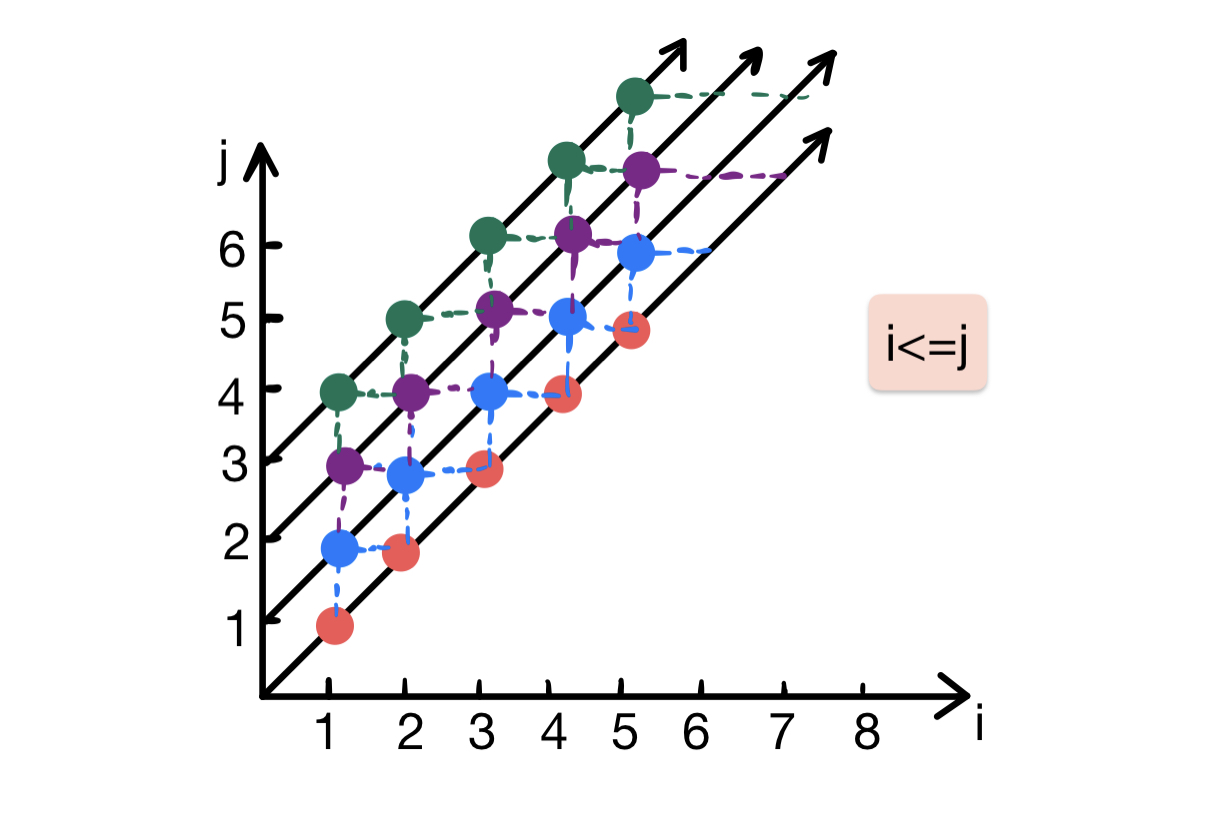
\includegraphics[width=0.4\textwidth]{Lab05-YanjieZe/axis3.jpg}
                \caption{Compute All $e[i,j]$}\label{axis3}
            \end{figure}
			
            Based on the computation path constructed before, we propose Alg.~\ref{alg1} \textbf{Optimal Binary Search Tree Bottom-up Dynamic Programming}. Line 1 to Line 6 is initialization. Line 7 to Line 9 is the implementation of the computation path.
            
            
            
            \begin{algorithm}[H]
               \caption{OBST Bottom-up DP}\label{alg1}
               \For{$i=0\rightarrow n$}
               {
                    $e[i+1,i]=q[i]$\;
                    $w[i+1,i]=q[i]$\;
               }
               \For{$i=1\rightarrow n$}
               {
                    \For{$j=i\rightarrow n$}
                    {
                        $w[i,j]=\sum_{l=i}^{j} p_{l}+\sum_{l=i-1}^{j} q_{l}$
                    }
               }
               
               \For{$k=0 \rightarrow n-1$}{
                \For{$i=1 \rightarrow n-k$}{
                    $e[i,i+k] = \min_{i\leq r\leq i+k}\{ e[i,r-1] + e[r+1, i+k] + w[i,i+k]\}$
               }
               }
               \Return $e[1,n]$
            			
        	\end{algorithm}
			\end{solution}
			\item Implement your proposed algorithm in C/C++ and analyze the time complexity. ({\color{blue}The framework Code-OBST.cpp is attached on the course webpage}). Give the minimum search cost calculated by your algorithm. The test case is given as following:
			\begin{table}[H]
				\setlength{\abovecaptionskip}{0cm}
				\setlength{\belowcaptionskip}{0.1cm}
				\centering		
				\begin{tabular}{|c|cccccccc|}
					\hline
					$ i $&0&1&2&3&4&5&6&7\\
					\hline
					$ p_{i} $&&0.04&0.06&0.08&0.02&0.10&0.12&0.14\\
					\hline
					$ q_{i} $&0.06&0.06&0.06&0.06&0.05&0.05&0.05&0.05\\
					\hline
				\end{tabular}
			\end{table}
			\begin{solution}
			~\\
			The algorithm is implemented in \textbf{Code-OBST.cpp}.
			
			The cost of the optimal binary search tree is: \textbf{3.12}, and the output of the program is shown in Fig.~\ref{result}.
			
			 \begin{figure}[htbp]
                \centering
                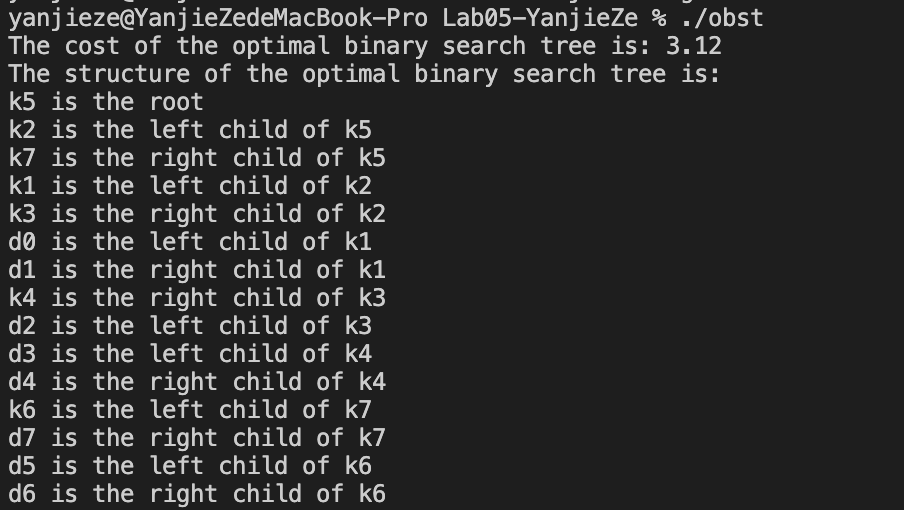
\includegraphics[width=0.4\textwidth]{Lab05-YanjieZe/result.png}
                \caption{Output of OBST Bottom-up DP}\label{result}
            \end{figure}
			
			~\\
			\textbf{Time Complexity}:$O(n^3)$
			
			From Line 1 to Line 3, time complexity is $O(n)$.
			
			From Line 4 to Line 6, the computation times are:
			\begin{equation}
			   \begin{split}
			\displaystyle t_1 &=  \sum_{i=1}^{n}\sum_{j=i}^{n}\left( (j-i+1)+(j-i+2) \right)\\
			& =  \sum_{i=1}^{n}\sum_{j=i}^{n}(2j-2i+3)\\
			&= \sum_{i=1}^{n} \{ (n-i)^2 + 4(n-i) + 3\} \\
			& = \frac 13 n^3 + \frac 32 n^2 + \frac 76 n \\
			& = O(n^3)
		      \end{split} 
			\end{equation}
			
			From Line 7 to Line 9, the computation times are:
			\begin{equation}
			    \begin{split}
			        \displaystyle t_2 &= \sum_{k=0}^{n-1}\sum_{i=1}^{n-k} k\\
			        &= \sum_{k=0}^{n-1}(nk-k^2)\\
			        &= \frac{n^3 - n}{6}\\
			        &= O(n^3)
			    \end{split}
			\end{equation}
			
			Therefore, overall time complexity is $O(n^3)$.
			
			~\\
			\textbf{Space Complexity}:$O(n^2)$
			
			In the algorithm we need two-dimensional arrays to store the middle results, which are $e, w$, and one-dimensional arrays, which are $p, q$.
			
			Then the space complexity is $O(n^2)$.
			
			\end{solution}
			\item Please draw the structure of the optimal binary search tree in the test case, and explain the drawing process.   
		\end{enumerate}
		    \begin{solution}
		    ~\\
	    Since we have gained $e[i,j]$ needed after running Alg.~\ref{alg1}, we can figure out what the optimal binary search tree is by utilizing $e[i,j]$.
	    
	    Here we do some changes on the original Alg.~\ref{alg1}. Define $root[i,j]$ as the root of the subtree containing $k_i,...,k_j$ and $d_{i-1},...,d_j$.
	    
	     \begin{algorithm}[H]
               \caption{OBST Bottom-up DP Modified}\label{alg2}
               \For{$i=0\rightarrow n$}
               {
                    $e[i+1,i]=q[i]$\;
                    $w[i+1,i]=q[i]$\;
               }
               \For{$i=1\rightarrow n$}
               {
                    \For{$j=i\rightarrow n$}
                    {
                        $w[i,j]=\sum_{l=i}^{j} p_{l}+\sum_{l=i-1}^{j} q_{l}$
                    }
               }
               
               \For{$k=0 \rightarrow n-1$}{
                \For{$i=1 \rightarrow n-k$}{
                    $e[i,i+k] = \min_{i\leq r\leq i+k}\{ e[i,r-1] + e[r+1, i+k] + w[i,i+k]\}$\;
                    $root[i,i+k] = r$\;
               }
               }
               \Return $e[1,n]$
            			
        	\end{algorithm}
        	
        Utilizing $root[i,j]$, we can easily use \textbf{First Order Traverse} to get each roor and node.
        
        Take the test case as an example:
        
        $root[1,7]=5\rightarrow k_5\ is\ the\ root$
        
        $root[1,5-1]=2 \rightarrow k_2\ is\ the\ left\ child\ of\ k_5$
        
        And the rest of the result is shown in Fig.~\ref{tree5}.
        
	    \begin{figure}[htbp]
                \centering
                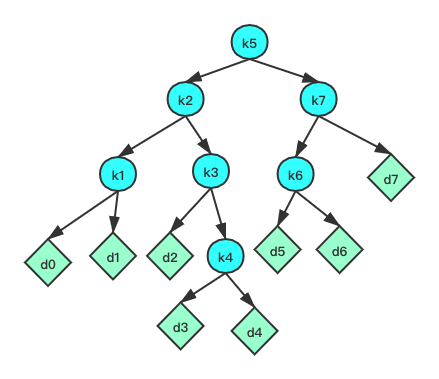
\includegraphics[width=0.4\textwidth]{Lab05-YanjieZe/tree5.png}
                \caption{Optimal Binary Search Tree (test)}\label{tree5}
            \end{figure}
	    \end{solution}
		
		\item \textit{Dynamic Time Warping Distance.} \textbf{DTW} stretches the series along the time axis in a dynamic way over different
		portions to enable more effective matching. Let $D T W(i, j)$ be the optimal distance between the first $i$ and first $j$ elements of two time series $\bar{X}=\left(x_{1} \ldots x_{n}\right)$ and $\bar{Y}=\left(y_{1} \ldots y_{m}\right),$ respectively. Note that the two time series are of lengths $n$ and $m$, which may not be the same. Then, the value of $D T W(i, j)$ is defined recursively as follows:
		$$
		DTW(i, j)=\left|x_{i}- y_{j}\right|+\min(DTW(i, j-1), DTW(i-1, j), DTW(i-1, j-1))
		$$
		
		\begin{enumerate}
			\item Implement the proposed DTW algorithm in C/C++ and analyze the time complexity of your implementation. ({\color{blue}The framework Code-DTW.cpp is attached on the course webpage}). Two test cases have been given in the source code. 
			\begin{solution}
			~\\
			Test result:0, 9.45455.
			
			The computation path of tabular Dynamic Programming is shown in Fig.~\ref{axis4}, which is different from the computation path shown in Fig.~\ref{axis3}. 
			
		
			
			 \begin{figure}[htbp]
                \centering
                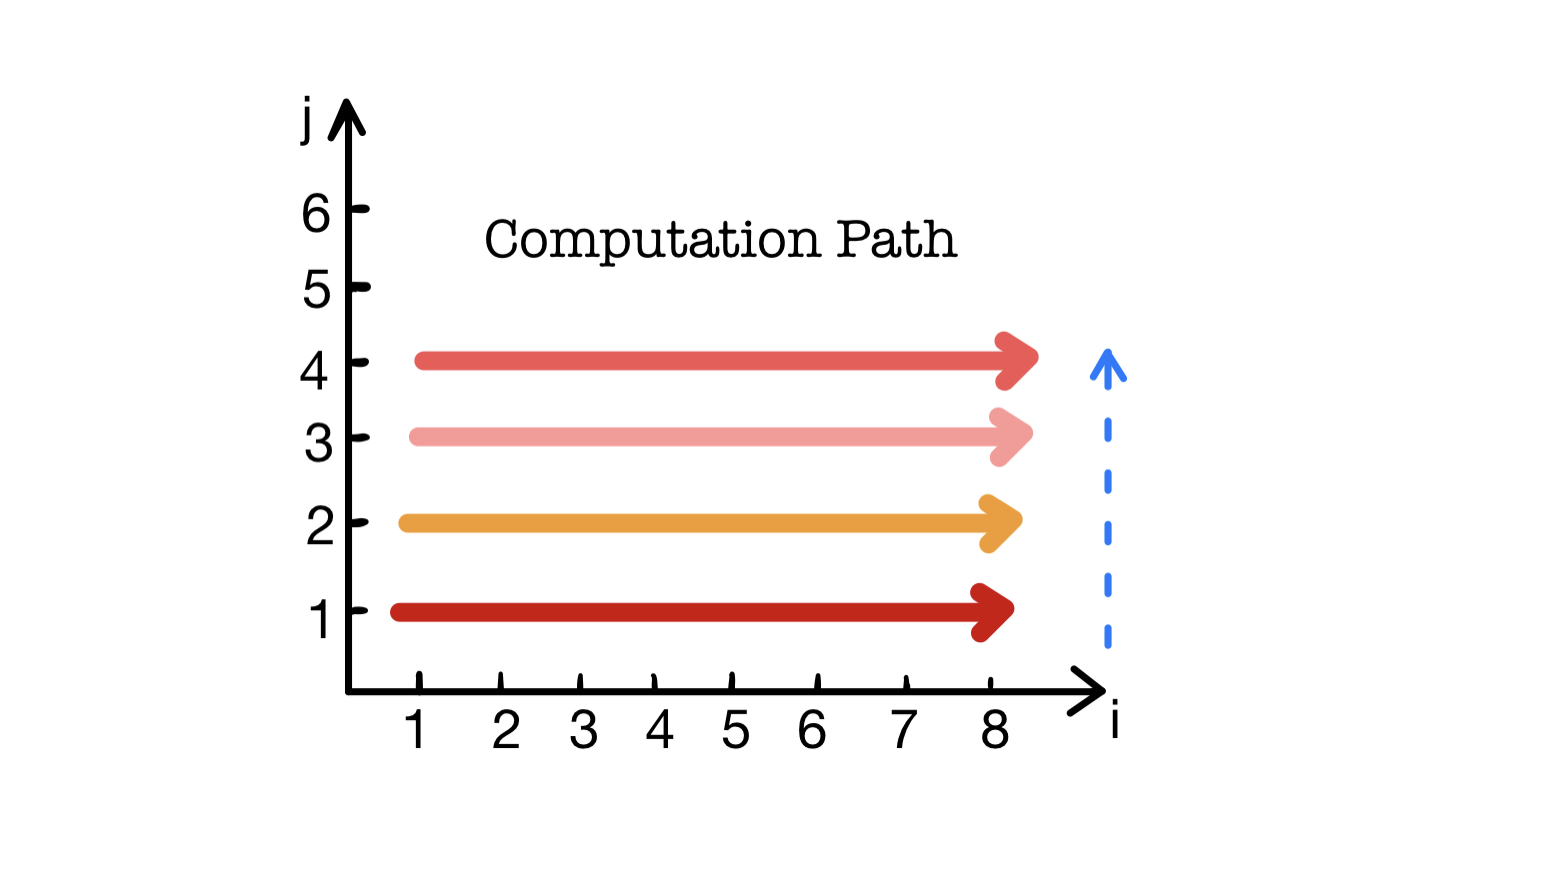
\includegraphics[width=0.4\textwidth]{Lab05-YanjieZe/axis4.jpg}
                \caption{Computation Path for DTW DP}\label{axis4}
            \end{figure}
			
			\textbf{Time Complexity:}$O(mn)$
			
			First, we need to initialize a cost matrix $DTW$, which has $O(mn)$ time complexity.
			
			Second, based on matrix $DTW$ we consume $O(m+n)$ time to find the minimal cost path, starting from the top right corner and traversing to bottom left.
			
			In total, Time Complexity is $O(mn)$.
			
			\end{solution}
			
			\item The window constraint imposes a minimum level $w$ of positional alignment between matched elements. The window constraint requires that $DTW(i, j)$ be computed only when $|i-j| \leq w$. Modify your code to add a window constraint and give the results of $ w=0 $ and $ w=1 $ on the two test cases. 
			\begin{solution}
			~\\
			When $window\ constraint = 0$, two results are 55.9286, 20.8889.
			
			When $window\ constraint = 1$, two results are 0, 13.9.
			
			The output of the program is shown in Fig.~\ref{result2} . (\textbf{Note}, when $window\ constraint$ is large, the result is the same as before).
			\begin{figure}[H]
			    \centering
			    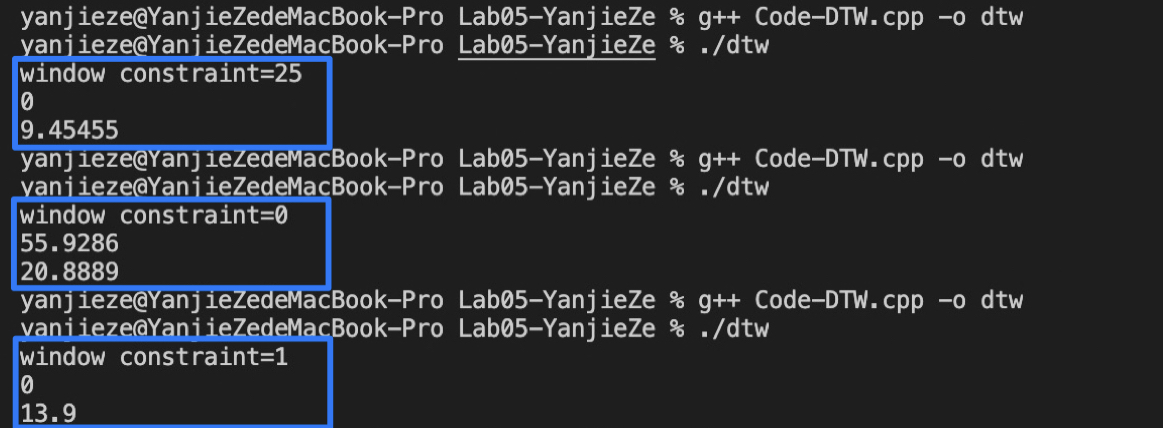
\includegraphics[width=0.6\textwidth]{Lab05-YanjieZe/result2.jpg}
			    \caption{Results for DTW}
			    \label{result2}
			\end{figure}
			\end{solution}
		\end{enumerate}
		
		
	\end{enumerate}
	
	\vspace{20pt}
	
	\textbf{Remark:} You need to include your .pdf and .tex and {\color{red}\emph{$2$}} source code files in your uploaded .rar or .zip file. Screenshots of test case results are acceptable.
	
	%========================================================================
\end{document}
